\section{Classifiers}
Classifiers are functions which map the input vector to some specific category. In the context of machine learning, we usually use a set of labelled data (known as training data) to fit a classifier. This fitted classifier, also known as model, can then be used to do predictions on unknown data. Many types of classifiers exist such as linear classifiers, support vector machines, decision trees and neural networks (Figure \ref{fig:classifier_comparision}). One special classifier built from an ensemble of decision trees called the Random forest classifier is used in this work. 

\subsection{Random forest}
A random forest is a classifier consisting of a collection of tree structured classifiers $\{h(x, \Theta_k), k=1, ...\}$ where the  $\{\Theta_k\}$ are independent, identically distributed random vectors and each tree casts a unit vote for the most popular class at input {x} \cite{breiman2001random}. For a given data, a number of decision trees $B$ are constructed using bootstrapping. Every time a new split is done, a subset $m$ of total vectors (features) $f$ is used, such that $m < f$. If $m = f$, this procedure is called bagging. In practise, usually, $m \approx \sqrt{f}$. Surprisingly, the number of trees, $B$, is not critical and setting this to a very high value will not lead to overfitting, which can be shown to be a consequence of strong law of large numbers \cite{james2013introductiontostatlearning, breiman2001random}. This also makes random forests more robust to noise and outliers than other classifiers. 

Typically, each bagged tree uses around two-third of training points. Out-of-bag (OOB) estimates can be computed by preforming predictions on the remaining one-third points. OOB errors reflect the generalisability of the model. For each feature, we can also compute the total reduction of Gini index by that feature at each tree split, where Gini index is defined by: 
\begin{equation*}
    G = \sum_{k=1}^{K}(p_{mk}(1-p_{mk}))
\end{equation*}
and is a measure of variance across $K$ classes for the proportion of training observations, $p_{mk}$, in the $m^{th}$ region that are from the $k^{th}$ class. This gives us the feature importance, sometimes called the Gini importance. However, it should be noted that $m$ features used for each split are actually random and is not based on feature importance at all. This seemingly deceptive strategy forces all the subsequent trees to not use the same strongest predictor, thus forcing a decorrelation among the trees. This makes the outputs less variable and more reliable \cite{james2013introductiontostatlearning}.

\begin{figure}[!hbtp]
\centerline{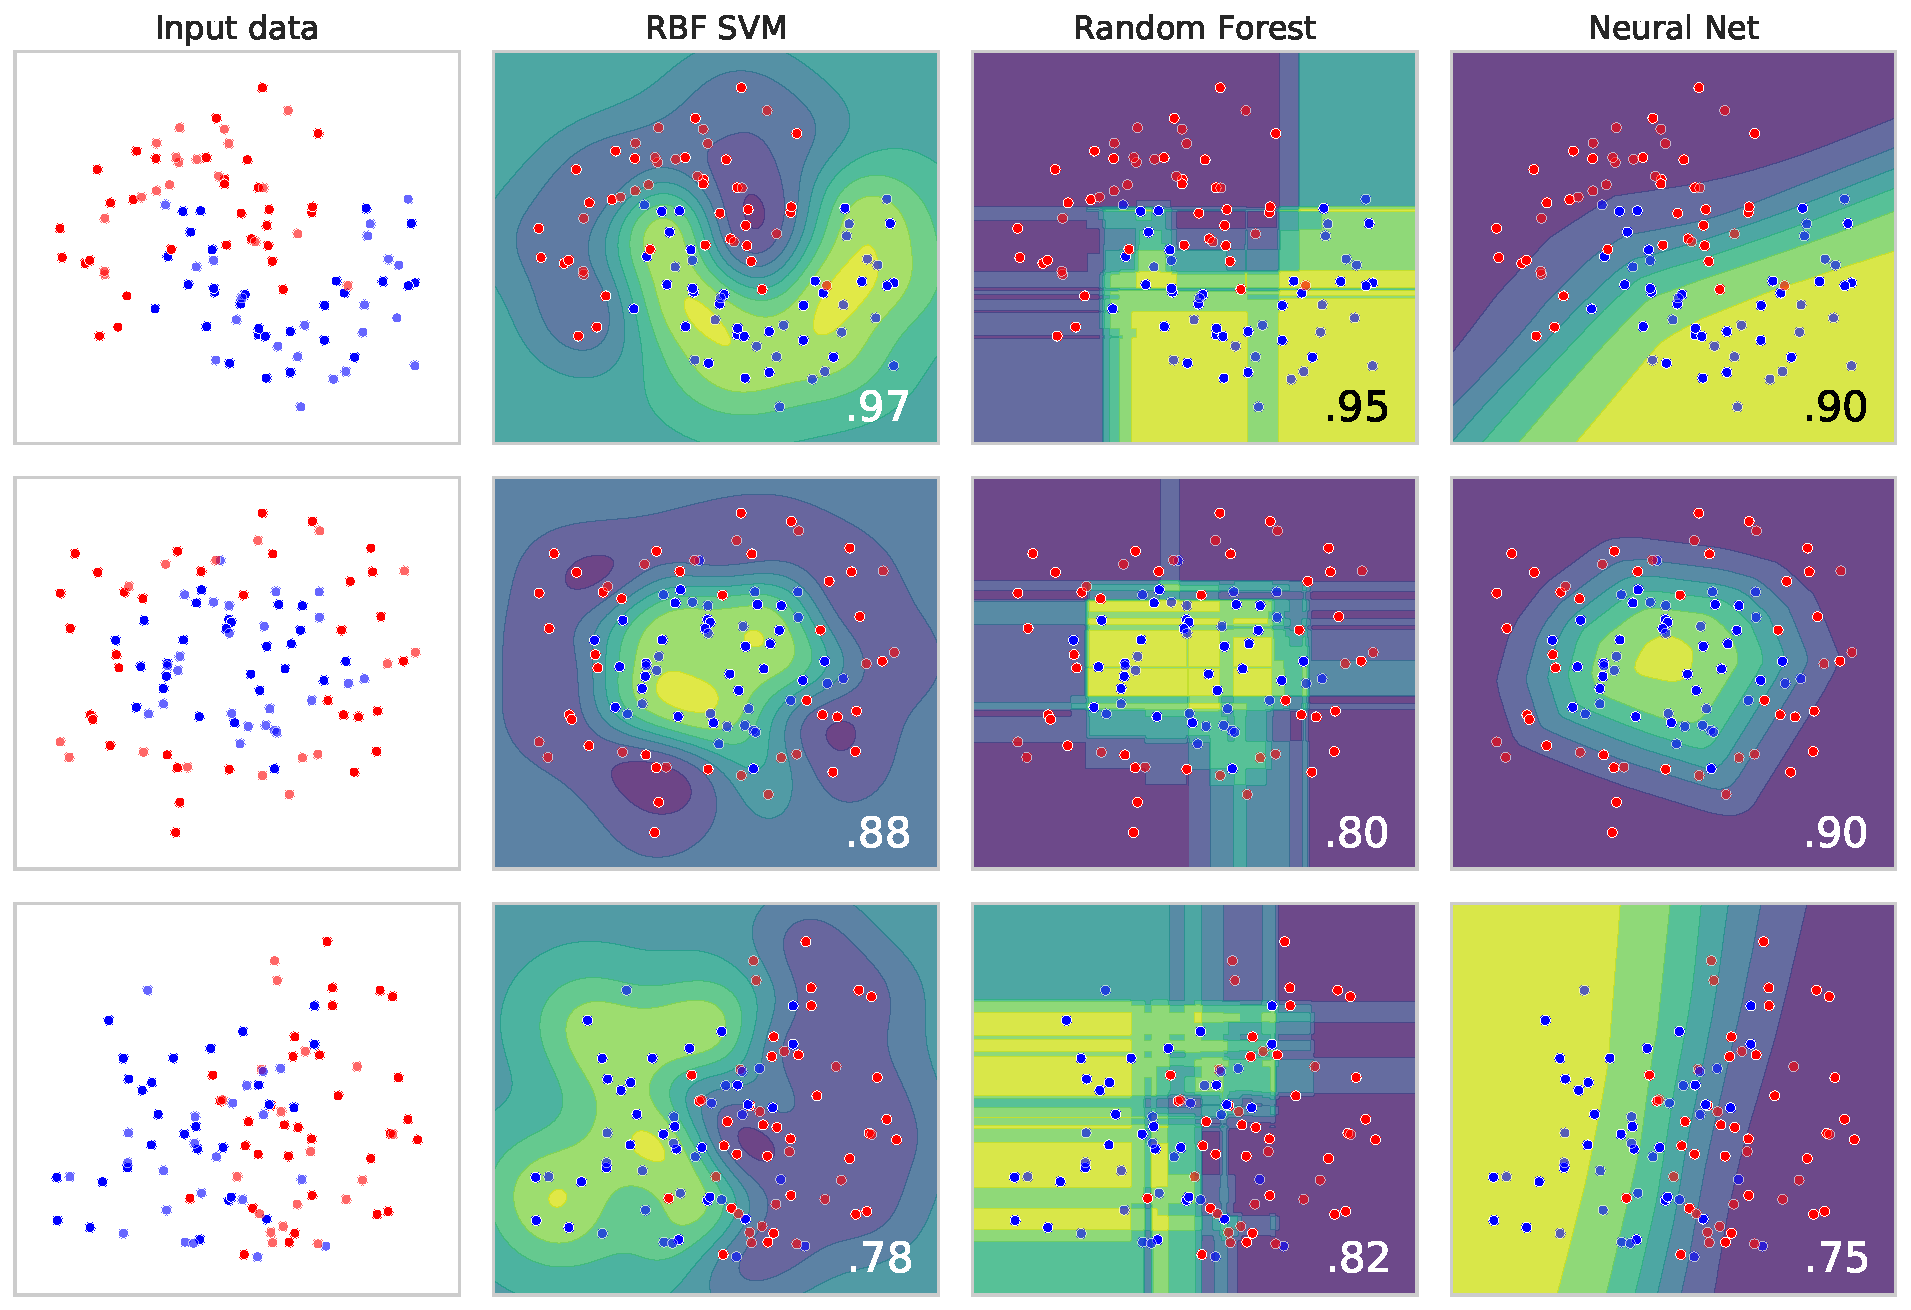
\includegraphics[width=1\textwidth]{chapters/Introduction/Figures/classifier_comparision.pdf}}
\caption[Comparison between some of the commonly used classifiers on synthetic datasets..]{{\bf Comparison between the some of the commonly used classifiers on synthetic datasets.} Three commonly used classifiers\textemdash SVM with RBF kernel, Random forest and a simple neural network (multi-layered perceptron) on three synthetic datasets as input. The input data is a binary data coloured as red and blue. The decision boundary is shown as contours and the accuracy of each classifier is shown on bottom right. Adapted from https://scikit-learn.org/stable/auto\_examples/classification/plot\_classifier\_comparison.html. SVM, Support Vector Machine; RBF, Radial Basis Function.}\label{fig:classifier_comparision}
\end{figure}